% ===== 05_inflection =====
\section{隔离控制函数的拐点分析}
\label{sec:s1:shape}
仅隔离控制的比例随时间严格下降，但下降速度未必单调。内部拐点可确定隔离比例下降最快的时刻；与前一节的成本和持续时间相比，它描述的是控制过程内部的时间分布。本节结果只针对 $c=c_0$ 的策略，不直接推广到任意联合控制。

\subsection{内部拐点及其相对位置}
\begin{theorem}
\label{thm:s1:inflection}
在条件\eqref{eq:model:trigger}下，$q_c(t)$ 在 $(t_1,t_2)$ 内存在唯一拐点，当且仅当
\begin{equation}
S_c<2\bar S<S^*,
\label{eq:s1:inflection-condition}
\end{equation}
等价地，$\frac12<(1-\beta)(1-q_0)<-\frac12W_{-1}(z_\eta)$。
内部拐点存在时，
\begin{equation}
S(t_{\rm inf})=2\bar S,\quad
 t_{\rm inf}=t_1+\frac{N}{c_0\eta}\ln\frac{S^*-\bar S}{\bar S},\quad
\qinf=1-\frac1{2(1-\beta)}.
\label{eq:s1:inflection-values}
\end{equation}
此时 $q_0<\qinf<q_{\max}$，且隔离比例的下降速度在 $t_{\rm inf}$ 唯一达到最大值。
\end{theorem}
\begin{proof}
对式\eqref{eq:s1:qprime}求导，得
\begin{equation}
\frac{d^2q_c(t)}{dt^2}
=\frac{\gamma c_0\eta^2}{\beta N}
\frac{(S-\bar S)(2\bar S-S)}{S^3}.
\label{eq:s1:qsecond}
\end{equation}
由于 $S>\bar S$，其符号由 $2\bar S-S$ 决定。$S$ 从 $S^*$ 严格下降至 $S_c$，所以恰在式\eqref{eq:s1:inflection-condition}成立时穿过 $2\bar S$，且只穿过一次。将该状态代入式\eqref{eq:s1:S-analytic}及\eqref{eq:s1:q-control}，即得时间和隔离比例。条件\eqref{eq:s1:inflection-condition}蕴含 $\beta<1/2$，故所列 $\qinf$ 表达式有定义。二阶导数先负后正，而一阶导数始终为负，故 $|dq_c/dt|$ 在该时刻达到唯一最大值。
\end{proof}

拐点处的隔离比例只依赖 $\beta$，但它出现的时间还取决于触发状态与控制持续时间。为比较其在各自控制区间内的位置，定义
\begin{equation}
\lambda=\frac{t_{\rm inf}-t_1}{t_2-t_1}
=\frac{\ln[(S^*-\bar S)/\bar S]}
{\ln[(S^*-\bar S)/(S_c-\bar S)]}\in(0,1).
\label{eq:s1:lambda}
\end{equation}
其中拐点前、后的两段时长分别为
\begin{equation}
t_{\rm inf}-t_1=\frac{N}{c_0\eta}\ln\frac{S^*-\bar S}{\bar S},\qquad
 t_2-t_{\rm inf}=\frac{N}{c_0\eta}\ln\frac{\bar S}{S_c-\bar S}.
\label{eq:s1:seg-high}
\end{equation}
$\lambda$ 较大表示下降最快的时刻相对靠后，不能据此判断绝对时刻 $t_{\rm inf}$ 的变化，也不将其解释为前后阶段累计放松量的比例。

若 $2\bar S\le S_c$，则 $q_c''(t)<0$ 对 $t\in(t_1,t_2)$ 成立；等号对应拐点到达控制终点。若 $2\bar S\ge S^*$，则 $q_c''(t)>0$ 对 $t\in(t_1,t_2)$ 成立；等号对应拐点到达控制起点。两种等号情形均无内部拐点。特别地，$\beta=1$ 时 $\bar S=0$，始终不存在内部拐点。

\subsection{相对位置的参数敏感性}
\label{sec:s1:inflection-position}
\begin{proposition}
\label{prop:s1:lambda-sensitivity}
在触发条件及 $S_c<2\bar S<S^*$ 下，固定其余参数，有
\[
\frac{\partial\lambda}{\partial\eta}<0,\qquad
\frac{\partial\lambda}{\partial c_0}>0,\qquad
\frac{\partial\lambda}{\partial\beta}>0.
\]
$\partial\lambda/\partial q_0$ 在允许参数域中可正可负，其驻点满足
\begin{equation}
\frac{\ln[(S^*-\bar S)/\bar S]}{(1-q_0)[\beta+q_0(1-\beta)]}
=-\frac{\ln[\bar S/(S_c-\bar S)]}{S^*-\bar S}
\frac{\partial S^*}{\partial q_0}.
\label{eq:s1:lambda-q0-stationary}
\end{equation}
\end{proposition}
\begin{proof}
记 $A=\ln[(S^*-\bar S)/\bar S]>0$、$B=\ln[\bar S/(S_c-\bar S)]>0$，则
\[
\frac{\partial\lambda}{\partial p}
=\frac{B\,\partial A/\partial p-A\,\partial B/\partial p}{(A+B)^2}.
\]
关于 $\eta$，$\partial A/\partial\eta=(\partial S^*/\partial\eta)/(S^*-\bar S)<0$，且 $\partial B/\partial\eta=0$。
关于 $c_0$，
\[
\frac{\partial A}{\partial c_0}=
\frac{\partial S^*/\partial c_0+S^*/c_0}{S^*-\bar S}>0,
\qquad \frac{\partial B}{\partial c_0}=0.
\]
关于 $\beta$，
\[
\frac{\partial A}{\partial\beta}
=\frac{\partial S^*/\partial\beta+S^*/[\beta(1-\beta)]}{S^*-\bar S}>0,
\qquad
\frac{\partial B}{\partial\beta}
=-\frac1{(1-\beta)[\beta+q_0(1-\beta)]}<0.
\]
这些符号给出前三个结论。最后，
\begin{equation}
\frac{\partial\lambda}{\partial q_0}
=\frac1{(A+B)^2}\left[
\frac{B}{S^*-\bar S}\frac{\partial S^*}{\partial q_0}
+\frac{A}{(1-q_0)[\beta+q_0(1-\beta)]}\right].
\label{eq:lambda-q0-sign}
\end{equation}
令方括号为零得到驻点条件。两项异号本身不足以证明导数能取两种符号；附录\ref{app:lambda}给出两个满足全部条件的参数点，并分别证明其导数为正和负。
\end{proof}

主要符号结果汇总于表\ref{tab:sensitivity}。对于 $q_0$，导数可以变号表示不存在覆盖整个允许参数域的统一方向，不表示每一条固定其他参数的曲线都非单调。
\begin{table}[htbp]
\centering\small
\setlength{\tabcolsep}{3.5pt}
\renewcommand{\arraystretch}{1.25}
\begin{threeparttable}
\caption{仅隔离控制中主要量的参数敏感性}
\label{tab:sensitivity}\label{tab:s1:lambda-sensitivity}\label{tab:s1:inflection-roles}
\begin{tabularx}{\linewidth}{@{}Xccccp{.24\linewidth}@{}}
\toprule
分析量 & $\beta$ & $q_0$ & $c_0$ & $\eta$ & 依据\\
\midrule
启动状态 $S^*$ & $>0$ & $<0$ & $>0$ & $<0$ & 引理\ref{lem:s1:Sstar-sensitivity}\\
控制持续时间 $\Delta t$ & $>0$ & $<0$ & 不定 & $<0$ & 命题\ref{prop:threshold-tradeoff}、\ref{prop:contact-effects}\\
拐点处隔离比例 $\qinf$ & $<0$ & $=0$ & $=0$ & $=0$ & 定理\ref{thm:s1:inflection}\\
拐点相对位置 $\lambda$ & $>0$ & 不定 & $>0$ & $<0$ & 命题\ref{prop:s1:lambda-sensitivity}\\
\bottomrule
\end{tabularx}
\begin{tablenotes}[flushleft]\footnotesize
\item 注：各单元格表示对列示参数求偏导的符号，固定初始状态、人口及其余参数。前两行要求控制被触发；后两行还要求内部拐点存在。不定指在所述参数域内没有统一符号。固定 $N$ 时以 $\theta=\eta/N$ 替换 $\eta$ 不改变符号。
\end{tablenotes}
\end{threeparttable}
\end{table}


% ===== 05_numerical_illustrations =====
\subsection{拐点的数值分析}

图~\ref{fig:s1:lambda-sensitivity} 给出 $\lambda$ 随 $\eta/N,c_0,\beta,q_0$ 的变化。
在内部拐点存在的范围内，$\lambda$ 随 $\eta$ 增大而减小，随 $c_0$ 和 $\beta$ 增大而增大，与命题~\ref{prop:s1:lambda-sensitivity} 一致。
固定 $N=763,S_0=762,I_0=1,\gamma=0.3504,c_0=10,\eta/N=0.05$，在 $q_0\in[0,0.39]$ 内得到以下局部极大值位置：
\[
\begin{array}{c|ccc}
\beta & 0.10 & 0.12 & 0.155\\
\hline
q_0^\dagger
&0.0736525&0.1969606&0.3890712
\end{array}
\]
这三个位置两侧的 $\frac{\partial \lambda}{\partial q_0}$ 均由正变负，且极大值位置随 $\beta$ 增大而增大。这是所考察参数范围内的数值结果，不涉及一般参数下驻点的唯一性。


\begin{figure}[htbp]
\centering
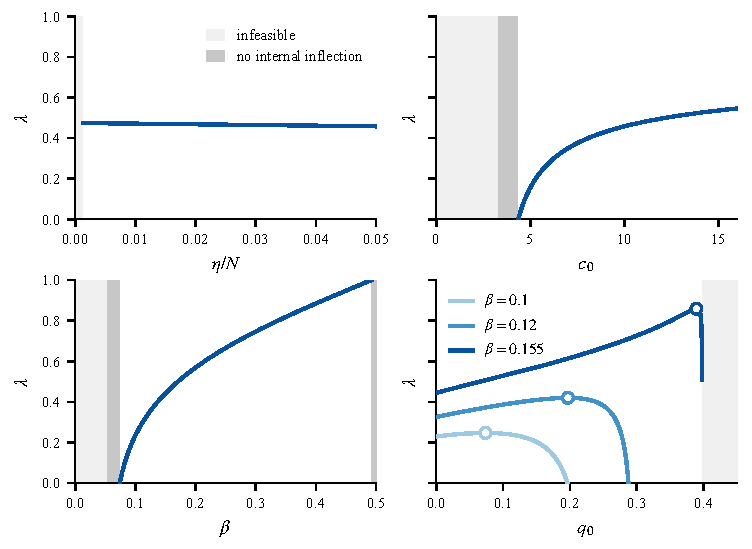
\includegraphics[width=0.8\textwidth]{figures/layout_v5/scenario1_inflection_lambda_sensitivity.pdf}
\caption{拐点相对位置 $\lambda$ 随 $\eta/N,c_0,\beta,q_0$ 的变化。基准取 $N=763,S_0=762,I_0=1,\beta=0.155,\gamma=0.3504,c_0=10,q_0=0.01526,\eta/N=0.05$；$q_0$ 面板另比较 $\beta=0.10,0.12,0.155$。空心圆表示数值局部极大值，浅灰区域表示不满足触发条件，深灰区域表示已触发控制但无内部拐点。$q_0$ 面板的灰色区域对应 $\beta=0.155$。}
\label{fig:s1:lambda-sensitivity}
\end{figure}


改变 $\beta$ 时，两端的拐点边界均可能出现；改变 $c_0$ 时，内部拐点在 $S^*=2\bar S$ 处出现。对于图示的 $q_0$ 和 $\eta/N$ 范围，只要满足控制触发条件，内部拐点就存在。由于 $\qinf$ 仅依赖于 $\beta$，其值在其余三个参数的比较中保持不变。相应的隔离率时间轨迹见图~\ref{fig:s1:inflection-scan}。


\begin{figure}[htbp]
\centering
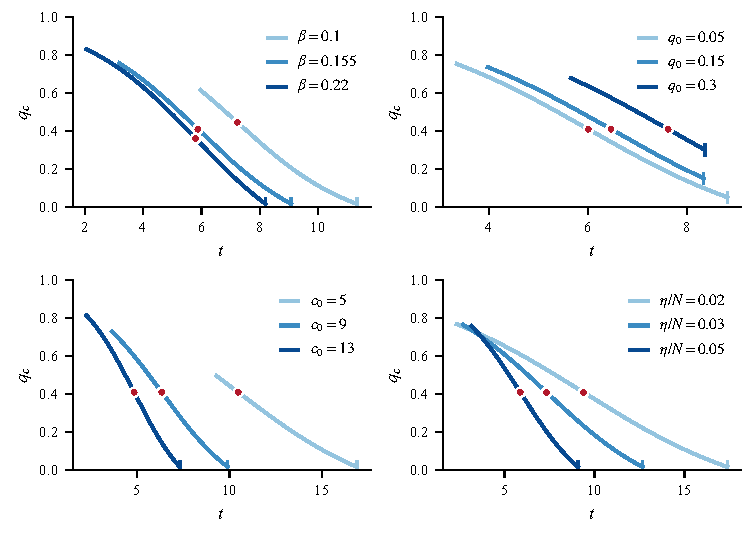
\includegraphics[width=0.8\textwidth]{figures/layout_v5/scenario1_inflection_scan_t.pdf}
\caption{不同 $q_0,\beta,c_0,\eta/N$ 下的隔离率时间轨迹。其余参数同图\ref{fig:s1:lambda-sensitivity}。圆点为内部拐点，短竖线为控制结束时刻 $t_2$。横轴 $t$ 的单位为天。}
\label{fig:s1:inflection-scan}
\end{figure}


附录~\ref{app:c0_beta} 给出了 $(c_0,\beta)$ 平面上的拐点存在范围。固定 $\theta=0.002$、$q_0=0.3230$ 时，西安参数 $(c_0,\beta)=(12.8872,0.1498)$ 位于该范围内。


\FloatBarrier

